\documentclass[conference,letterpaper]{IEEEtran}
\IEEEoverridecommandlockouts
\usepackage{amssymb,amsmath,graphicx,float,array,theorem}
\usepackage[noadjust]{cite}
\usepackage[latin1]{inputenc}
% hyperref is not recommended for work submitted to IEEE - Walter
%\usepackage[dvips,ps2pdf]{hyperref}

\newcommand\real{\mathbb{R}}
\newcommand{\req}[1]{(\ref{#1})}
\DeclareMathOperator{\atan}{atan2}

%\overrideIEEEmargins
%\usepackage{multirow}
%\usepackage[left=0.71in,top=0.94in,right=0.71in,bottom=1.18in]{geometry}
%\setlength{\columnsep}{0.24in}

\begin{document}

\title{Point Stabilization of Mobile Robots with Nonlinear Model Predictive Control}

\author{\authorblockN{Felipe K\"{u}hne, Walter Fetter Lages and Jo\~{a}o Manoel Gomes da Silva Jr.}
\authorblockA{
\textit{Electrical Engineering Department} \\
\textit{Federal University of Rio Grande do Sul} \\
\textit{Av. Oswaldo Aranha, 103} \\
\textit{Porto Alegre, RS 90035-190 Brazil} \\
\{kuhne,fetter,jmgomes\}@eletro.ufrgs.br}}

\maketitle

\begin{abstract}
This paper presents an optimal control scheme based on model-based predictive control (MPC) for a wheeled mobile robot (WMR) with nonholonomic constraints. It is shown that, by using MPC, some advantages can be obtained, such as the ability to handle constraints due to state or input limitations and performance improvement. To solve some problems with other MPCs for WMRs, this paper proposes to formulate a cost function in polar coordinates. Considerations regarding the computational effort of the MPC are developed with the purpose of analysing the viability of the proposed technique in real-time.
\end{abstract}
\begin{keywords}
Nonholonomic systems, wheeled mobile robots, model-based predictive control.
\end{keywords}

%%%%%%%%%%%%%%%%%%%%%%%%%%%%%%%%%%%%%%%
\section{Introduction}\label{sec:intro}

The field of mobile robot control has been the focus of active research in the past decades. Despite the apparent simplicity of the kinematic model of a wheeled mobile robot (WMR), the design of stabilizing control laws for those systems can be considered a challenge due to the existence of nonholonomic constraints. Due to Brockett's conditions~\cite{brockett82}, a smooth static state feedback control law cannot be used to stabilize a nonholonomic system at a given configuration. To overcome these limitations traditional techniques use non-smooth or time-varying control laws~\cite{bloch89,samson91,canudas92,yamamoto94,murray97}.

However, in realistic implementations, the traditional techniques for the control of nonholonomic WMRs often do not present good results, due to constraints on inputs or states that naturally arise. Also, in general, the resulting closed-loop trajectory presents unnecessary oscillatory motions. Furthermore, tuning parameters are difficult to choose in order to achieve good performance since the control laws are not intuitively obtained.

In this paper we show that, by using model-based predictive control (MPC), these disadvantages can be overcome: the tuning parameters are easy to deal with; a cost function is minimized, which makes the control law optimal according to the optimization criterion; constraints on state and control inputs can be considered in a straightforward way. Note that for a WMR the latter is an important feature, since the position of the robot can be restricted to belong to a safe region. Control actions that respect actuators limits can be generated. Furthermore, a control law that respects Brockett's conditions can be implicitly obtained.

On the other hand, the main drawback of MPC schemes is related to its computational burden which, in the past years, had limited its applications only to sufficient slow dynamic systems. However, with the development of increasingly faster processors and efficient numerical algorithms, the use of MPC in faster applications which is the case of WMRs becomes possible. 

Although MPC is not a new control method, works dealing with MPC of WMRs are
sparse. In~\cite{ollero91,rico99}, GPC (Generalized Predictive Control) is
used to solve the path following problem. A linear model is used to compute
the distance between the robot and a reference path. The control acts only
in the angular velocity, while the linear velocity is constant.
In~\cite{ortega96} a nonlinear model of the WMR is used for trajectory
tracking. The problem is solved considering unknown obstacles in the
configuration space. A neural network is used in the optimization problem.
In~\cite{yang98} the path following problem is solved. Neural networks are
used in the kinematic model which predicts the future behavior of a car-like
WMR. The modeling errors are corrected on-line with the neural network
model. Using a nonlinear model of the robot, in~\cite{essen01} a nonlinear
MPC (NMPC) algorithm in state-space representation is developed, which is
applied to both problems of point stabilization and trajectory tracking. A
steady-state error is identified and a modified cost function to be
minimized is proposed. The disadvantages of the above cited works is that,
with a linear model, the problem of point stabilization can not be solved.
Furthermore, this model is only valid when the robot is close enough to the
reference path. Techniques using neural networks depends on training. Then,
the feasibility of the control law can not be guaranteed for all possible
situations. By using the controller proposed by~\cite{essen01}, it can be
noted that the steady-state error can not be totally eliminated.

In this paper a NMPC strategy is developed to solve the problem of point
stabilization for a nonholonomic WMR. By using a standard quadratic cost
function in the optimization problem, a large steady-state error in the
final configuration of the WMR is identified, caused by a coupling between
the position states of the kinematic model. By using the idea developed
in~\cite{essen01} which uses a modified cost function, this error is reduced
but not eliminated, since the coupling of the position states remains.
Therefore, in order to eliminate this steady-state error and also to improve
the performance of the closed-loop trajectories, a transformation to polar
coordinates which promotes the decoupling of the position states is
introduced in the cost function to be minimized. Also, computational effort
analysis are carried out to study the viability of the application of the
proposed algorithms in real-time.


%%%%%%%%%%%%%%%%%%%%%%%%%%%%%%%%%%%%%%%%%%%%%%%%%%%%%
\section{Kinematic Model of the WMR}\label{sec:model}

A mobile robot made up of a rigid body and non deforming wheels is considered (Fig.~\ref{fig:robot}). It is assumed that the vehicle moves without slipping on a plane, i.e., there is a pure rolling contact between the wheels and the ground. The kinematic model of the WMR is then given by~\cite{Campion:TRA-12-1}:
\begin{equation}\label{eqn:model}
	\left\{
		\begin{aligned}
			\dot x	  &= v\cos\theta \\
			\dot y	  &= v\sin\theta \\
			\dot \theta &= w
		\end{aligned}
	\right.
\end{equation}
where ${\bf x}=[x~~y~~\theta]^T$ describes the configuration (position and orientation) of the center of the axis of the wheels, $C$, with respect to a global inertial frame $\{O,X,Y\}$. ${\bf u}=[v~~w]^T$ is the control input, where $v$ and $w$ are the linear and the angular velocities, respectively.
\begin{figure}[b]
	\centering
	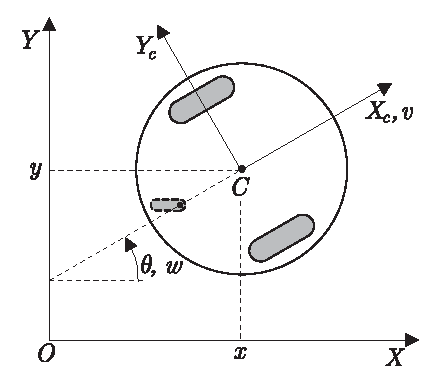
\includegraphics[width=0.58\linewidth]{Figures/robot.eps}
	\caption{Coordinate system of the WMR.}
	\label{fig:robot}
\end{figure}

%For the sake of simplicity, we assume in this work that the states of the plant are available for measurement and that there are no plant/model mismatch.

Since the MPC scheme used here is computed in discrete-time, it is necessary to discretize the kinematic model. Considering a sampling period $T$, a sampling instant $k$ and applying the Euler's approximation to~\req{eqn:model}, we obtain the following discrete-time model for the robot dynamics:
\begin{equation}
\label{eqn:discretemodel}
	\left\{
		\begin{aligned}
			x(k+1)	    &= x(k) + v(k)\cos\theta(k)T \\
			y(k+1)	    &= y(k) + v(k)\sin\theta(k)T \\
			\theta(k+1) &= \theta(k) + w(k)T \\
		\end{aligned}
	\right.
\end{equation}
or, in the compact representation,
\begin{equation}\label{eqn:discretemodelshort}
	{\bf x}(k+1) = f_d({\bf x}(k),{\bf u}(k)),
\end{equation}


%%%%%%%%%%%%%%%%%%%%%%%%%%%%%%%%%%%%%%%%%%
\section{The MPC Algorithm}\label{sec:mpc}

MPC is an optimal control strategy that uses the model of the system to obtain an optimal control sequence by minimizing an objective function. At each sampling instant, the model is used to predict the behavior of the system over a prediction horizon. Based on these predictions, the objective function is minimized with respect to the future sequence of inputs, thus requiring the solution of a constrained optimization problem for each sampling instant. Although prediction and optimization are performed over a future horizon, only the values of the inputs for the current sampling interval are used and the same procedure is repeated at the next sampling instant using the updated process measurements and a shifted horizon. This mechanism is known as {\it moving} or {\it receding horizon} strategy, in reference to the way in which the time window shifts forward from one sampling instant to the next one.

%In practice, every system is subject to constraints. The actuators have a limited field of action as well as a determined slew rate. Constructive reasons, safety or environmental ones or even sensor ranges can limit the system variables. Therefore the introduction of constraints in the problem becomes necessary.

Considering a robot described by~\req{eqn:discretemodelshort}, the following prediction model can be formulated:
\begin{equation*}
	{\bf x}(k+j+1|k)=f_d({\bf x}(k+j|k),{\bf u}(k+j|k)), ~~~j\in[0,N-1],
\end{equation*}
where $j\in[0,N-1]$ and the notation $a(m|n)$ indicates the value of $a$ at the instant $m$ predicted at instant $n$. Furthermore, we consider the existence of bounds on the amplitude of state and control variables:
\begin{align}
	\underline{\bf x} \leq {\bf x}(k+j|k) &\leq \overline{\bf x}, ~~~j\in[0,N],\label{eqn:restx} \\
	\underline{\bf u} \leq {\bf u}(k+j|k) &\leq \overline{\bf u}, ~~~j\in[0,N-1],\label{eqn:restu}
\end{align}
where $\underline{\bf x}$ and $\underline{\bf u}$ stand for lower bounds and $\overline{\bf x}$ and $\overline{\bf u}$ stands for the upper bounds\footnote{The symbol $\leq$ stands for componentwise inequalities in this case.}.  

The cost function to be minimized can be stated as a quadratic function of the states and control inputs:
\begin{multline}\label{eqn:cost}
	\Phi(k) = \sum_{j=1}^{N}{\bf x}^T(k+j|k){\bf Q}{\bf x}(k+j|k) + \\ + {\bf u}^T(k+j-1|k){\bf R}{\bf u}(k+j-1|k),
\end{multline}
which will be called hereafter the original cost function in cartesian coordinates, where $N$ is the prediction horizon and ${\bf Q}\geq 0$, ${\bf R}>0$ are weighting matrices used to penalize the state error and the control effort, respectively.

The optimization problem can therefore be stated as to find a sequence of states and controls such that:
\begin{equation}\label{eqn:optim}
	{\bf x}^\star,{\bf u}^\star = \arg\min_{{\bf x},{\bf u}}\left\{\Phi(k)\right\} \\
\end{equation}
s. a.
\begin{alignat}{2}
	{\bf x}(k|k)     &= {\bf x}_0, \label{eqn:restci} \\
	{\bf x}(k+j+1|k) &= f_d({\bf x}(k+j|k),{\bf u}(k+j|k)), ~&j &\in[0,N-1] \label{eqn:restmodel} \\
	{\bf Cx}(k+j|k)  &\leq {\bf c}, ~~j \in[0,N] \label{eqn:restx1} \\
	{\bf Du}(k+j|k)  &\leq {\bf d}, ~~j \in[0,N-1] \label{eqn:restu1}
\end{alignat}
where ${\bf x}_0$ in~\req{eqn:restci} is the initial condition which
corresponds to the value of the states measured at the current instant.

Constraint~\req{eqn:restmodel} represents the prediction model
and~\req{eqn:restx1}-\req{eqn:restu1} are a general form to represent
linear bounds in the state and control variables, and they may be present
or not in the optimization problem. Note that we can
rewrite~\req{eqn:restx1}-\req{eqn:restu1} in the form
of~\req{eqn:restx}-\req{eqn:restu} with: 
\begin{equation*}\label{eqn:const2}
	{\bf C} = {\bf D} = \begin{bmatrix} {\bf I} \\ -{\bf I} \end{bmatrix}, \quad 
	{\bf c} = \begin{bmatrix} \overline{\bf x} \\ -\underline{\bf x} \end{bmatrix}, \quad
	{\bf d} = \begin{bmatrix} \overline{\bf u} \\ -\underline{\bf u} \end{bmatrix}	
\end{equation*}

The optimization problem~\req{eqn:optim}--\req{eqn:restu1} is then solved at each time step $k$, yielding a sequence of optimal states $\{{\bf x}^\star(k|k+1),\cdots,{\bf x}^\star(k+N|k)\}$, optimal control inputs $\{{\bf u}^\star(k|k),\cdots,{\bf u}^\star(k+N-1|k)\}$ and the optimal cost $\Phi^\star(k)$. The MPC control law is implicitly given by the first control action of the sequence of optimal control, ${\bf u}^\star(k|k)$, and the remaining portion of this sequence is discarded.


%%%%%%%%%%%%%%%%%%%%%%%%%%%%%%%%%%%%%%%%%%%%%%%%%%%%%%%%%%%%%%%%%%%%%%%%%%%%%%
\section{MPC with Cost Function in Cartesian Coordinates}\label{sec:cartesian}

In this section we focus on the formulation of MPC for the WMR considering a cost function in cartesian coordinates. In order to evaluate the performance of the approach, simulation results are shown\footnote{All the optimization problems of this paper has been solved with the {\sc Matlab} routine {\tt fmincon}.}. As a case study, let us consider the robot Twil~\cite{lages98a}, which have the following limits in the amplitude of the control variables~\cite{kuhne05}:
\begin{equation}\label{eqn:const}
	\underline{\bf u} = \begin{bmatrix}-0.47~m/s\\-3,77~rad/s\end{bmatrix} \qquad \overline{\bf u} = \begin{bmatrix}0.47~m/s\\3.77~rad/s\end{bmatrix}
\end{equation}

Initially, the cost function to be minimized is that showed in~\req{eqn:cost}. Then, a second case with some modifications to the cost function, proposed in~\cite{essen01}, is shown. In both cases, constraints only in the amplitude of the control inputs based on the robot Twil, Eq.~\req{eqn:const} will be taken into account.

\subsection{Original Cost Function in Cartesian Coordinates.}\label{sec:pure}
The weighting matrices used here are ${\bf Q}={\rm diag}(1,1,0.5)$ (equal penalty in the position states and a half of the penalty in the orientation) and ${\bf R}={\rm diag}(0.1,0.1)$ (less penalty in the control effort). The prediction horizon is $N=5$. The initial configuration is \mbox{${\bf x}_0=[0~~6~~0]^T$}, and the goal is the origin. The obtained simulation results are shown in Figures~\ref{fig:traj_01}-\ref{fig:control_01}.
\begin{figure}[htbp]
	\centering
    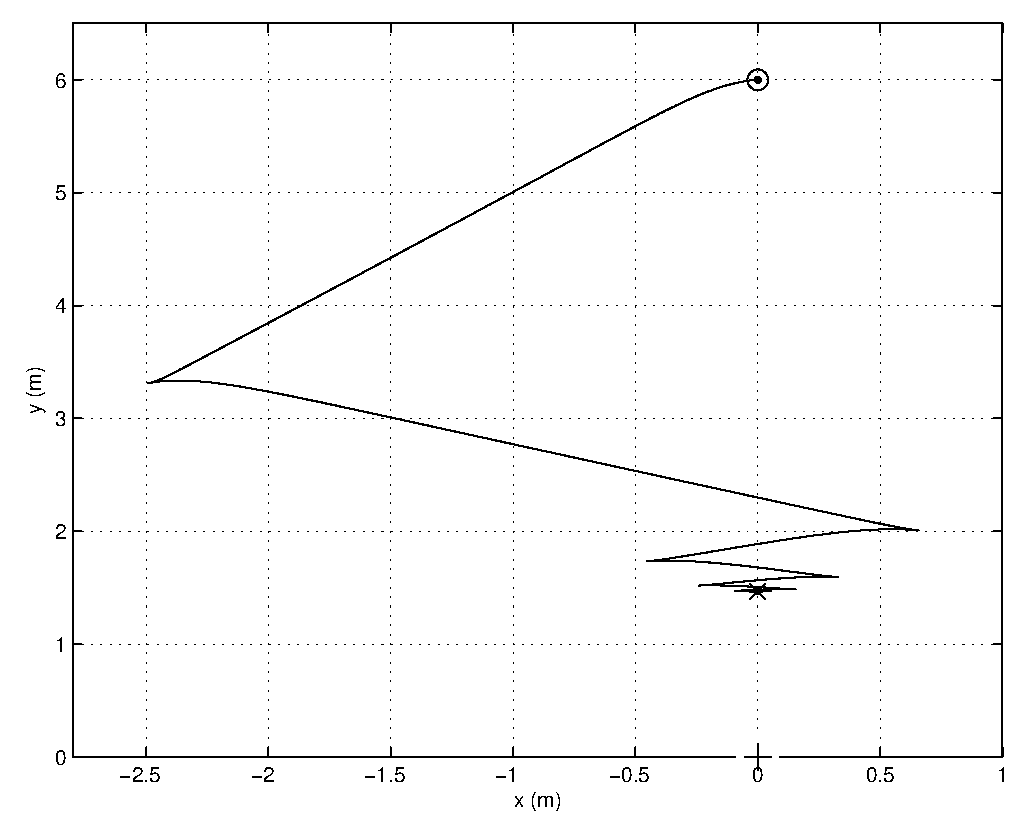
\includegraphics[width=.82\linewidth]{Figures/traj_01.eps}
    \caption{Trajectory in the XY-plane.}
    \label{fig:traj_01}
\end{figure}
\begin{figure}[htbp]
	\centering
    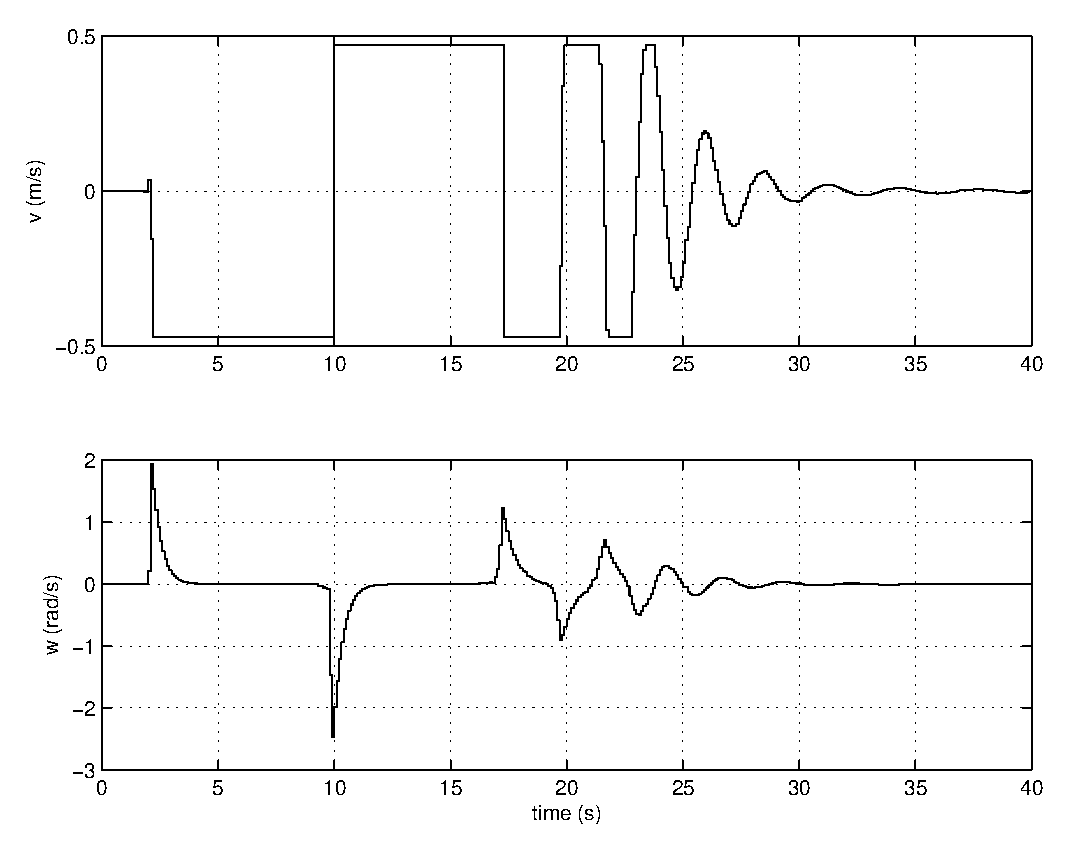
\includegraphics[width=.82\linewidth]{Figures/control_01.eps}
    \caption{Control inputs.}
    \label{fig:control_01}
\end{figure}

Fig.~\ref{fig:traj_01} shows the trajectory of the robot in the XY-plane and
Fig.~\ref{fig:control_01} shows that the generated control signals respect
the imposed constraints. It is easy to note that there is a large
steady-state error in one of the position variables ($y$-state, in this
case). Notice also that the robot has already stopped since both control
inputs converge to zero. The final configuration is ${\bf
x}_f=[0~~1.47~~0]^T$. This steady-state error can be explained by the fact
that both states, $x$ and $y$, depends on the same control variable, the
linear velocity $v$, as seen in~\req{eqn:model}. Thus, when the optimization
algorithm minimizes with respect to $v$ and $x$, it can no more minimize
with respect to $y$, since the cost function obeys a monotonic decreasing
behavior. In~\cite{kuhne05} is shown that, by increasing considerably the
prediction horizon, this problem can be reduced. However, long prediction
horizons are in general undesirable since the computational effort is
directly related to it.

\subsection{Modified Cost Function in Cartesian Coordinates.}\label{sec:essen}
The steady-state error presented in Section~\ref{sec:pure} was also identified in~\cite{essen01}. In the attempt of eliminating it, a modified cost functions have been proposed in order to increase the state penalty over the horizon, thus forcing the states to converge to an acceptable solution. Hence, the idea of exponentially increasing state weighting has been introduced. Also, a terminal state cost has been added to the cost function to be minimized. From these modifications the cost function assumes therefore the following form:
\begin{multline}\label{eqn:essen_cost}
	\Phi(k) = \sum_{j=1}^{N-1}{\bf x}^T(k+j|k){\bf Q}(j){\bf x}(k+j|k) + \\ + \sum_{j=0}^{N-1}{\bf u}^T(k+j|k){\bf R}{\bf u}(k+j|k) + \Omega({\bf x}(k+N|k)),
\end{multline}
where $\Omega({\bf x}(k+N|k)) = {\bf x}^T(k+N|k){\bf P}{\bf x}(k+N|k)$ and ${\bf Q}(j) = 2^{j-1}{\bf Q}$.
Using the same tuning parameters and the same initial condition as in Section~\ref{sec:pure}, and with a terminal state weighting of ${\bf P}=50{\bf Q}(N)$, the simulation results are shown in Figures~\ref{fig:traj_02}-\ref{fig:control_02}.
\begin{figure}[htbp]
	\centering
	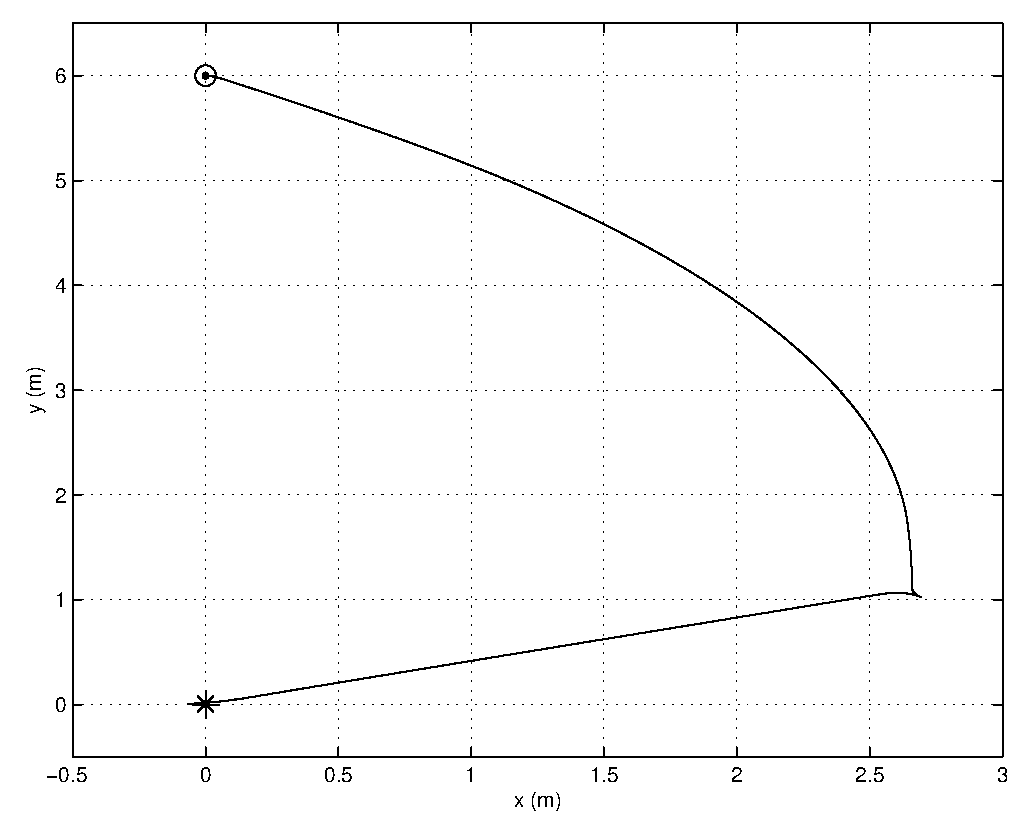
\includegraphics[width=.82\linewidth]{Figures/traj_02.eps}
   	\caption{Trajectory in the $XY$ plane.}
   	\label{fig:traj_02}
\end{figure}
\begin{figure}[htbp]
	\centering
   	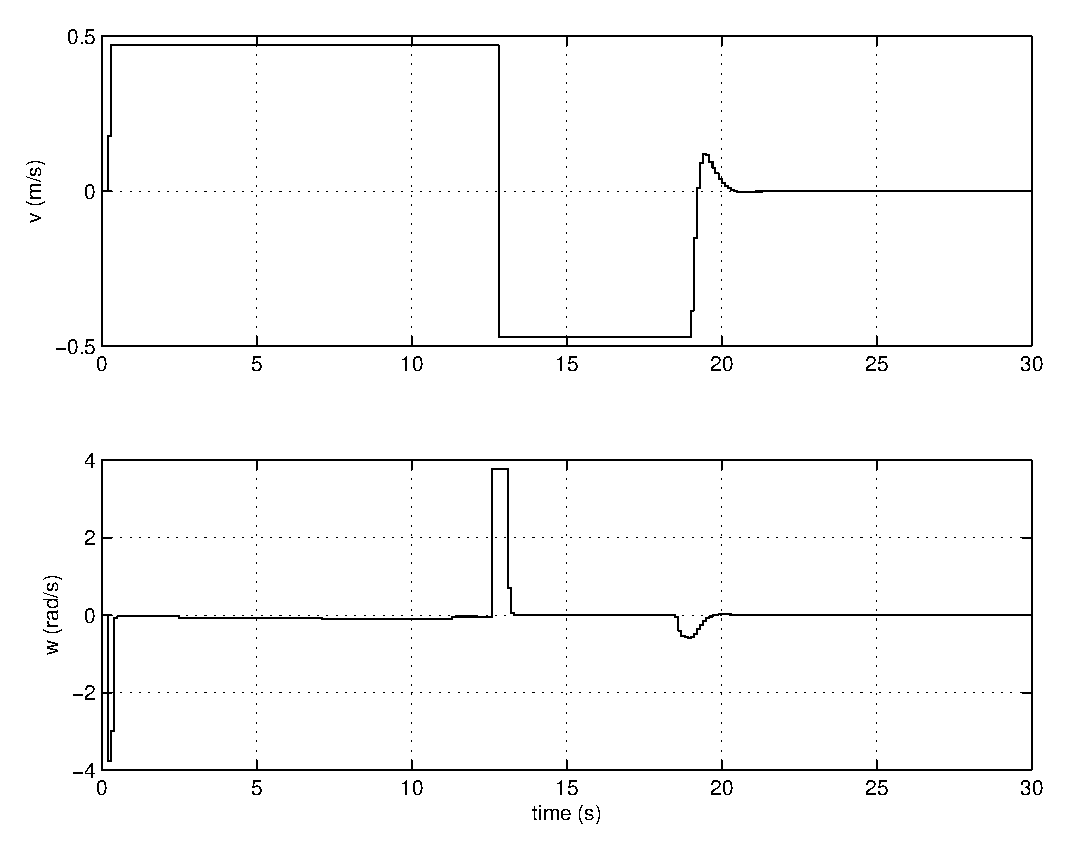
\includegraphics[width=.82\linewidth]{Figures/control_02.eps}
   	\caption{Control inputs.}
   	\label{fig:control_02}
\end{figure}

It can be seen in Fig.~\ref{fig:traj_02} that the large steady-state error in $y$-state has disappeared. Also, notice in Fig.~\ref{fig:control_02} that the convergence rate is higher. In the example of Section~\ref{sec:pure} the stabilization time is about 40 s, while here it is 21 s. Again, the control signals respect the imposed constraints.

However, even if it can be considered small, the final $y$-state still presents a persistent steady-state error since the coupling between the states $x$ and $y$ remains. The final configuration is ${\bf x}_f=[0~~0.006~~0]^T$. 


%%%%%%%%%%%%%%%%%%%%%%%%%%%%%%%%%%%%%%%%%%%%%%%%%%%%%%%%%%%%%%%%%%%%%%
\section{MPC with Cost Function in Polar Coordinates}\label{sec:polar}

Hence, a possible way to overcome the state steady-state error would be the use of some coordinate transformation able to decouple the position states $x$ and $y$ from the same control input, $v$. This idea is developed here, by using the following state transformations to polar coordinates, as proposed in~\cite{lages98b}:
\begin{equation*}
	e = \sqrt{x^2+y^2}, \qquad 
	\phi = \atan(y,x), \qquad
	\alpha = \theta - \phi,
\end{equation*}

In~\cite{lages98b}, it can be seen that, if one of the state variables converges to the origin, the other ones will also converge to the origin. Then the objective here is to incorporate this behavior in the cost function to be minimized. By defining ${\bf x}_p=[e~~\phi~~\alpha]^T$, the following cost function can be formulated:
\begin{multline}\label{eqn:polar_cost}
	\Phi_p(k) = \sum_{j=1}^{N}{\bf x}_p^T(k+j|k){\bf Q}{\bf x}_p(k+j|k) + \\ + {\bf u}^T(k+j-1|k){\bf R}{\bf u}(k+j-1|k)
\end{multline}

\subsection{NMPC with Constraints only in Control Variables.}
Changing the cost function in~\req{eqn:optim} by \req{eqn:polar_cost} and considering the same tuning parameters and initial condition used in Section~\ref{sec:cartesian}, the following results shown in Figures~\ref{fig:traj_03}-\ref{fig:control_03} are obtained. Once more, constraints in the amplitude of the control inputs described by~\req{eqn:const} are taken into account.
\begin{figure}[htbp]
	\centering
	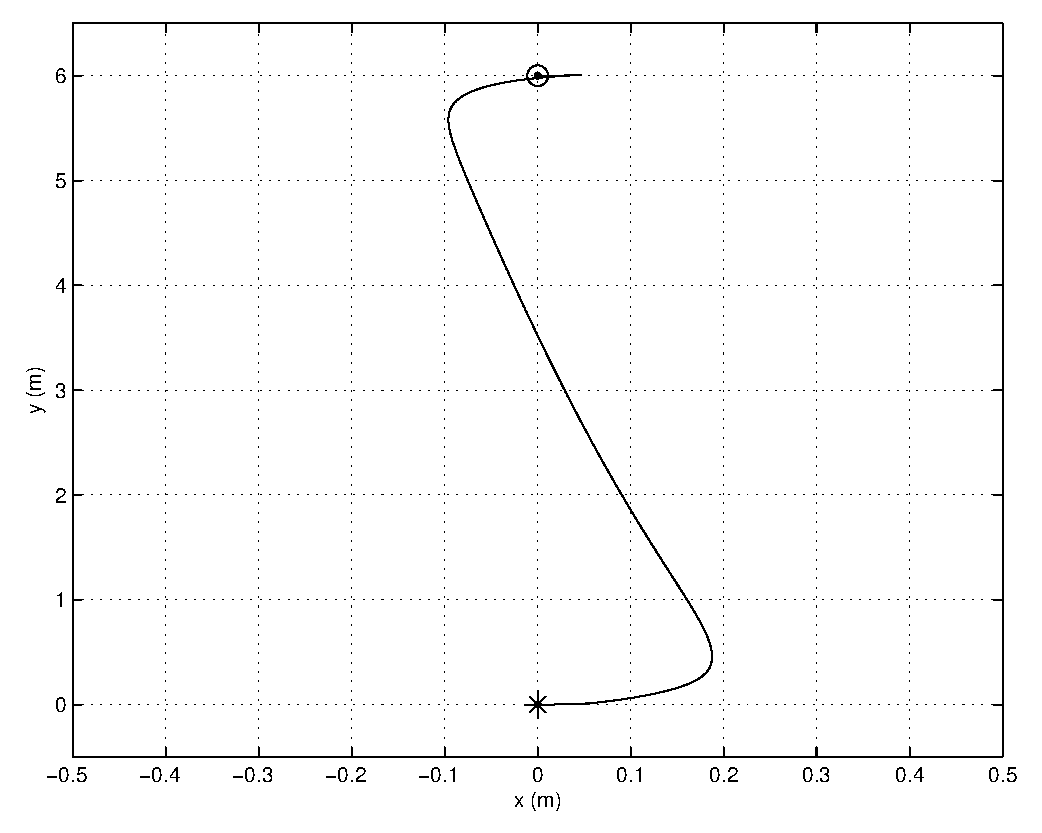
\includegraphics[width=.82\linewidth]{Figures/traj_03.eps}
   	\caption{Trajectory in the $XY$ plane.}
   	\label{fig:traj_03}
\end{figure}
\begin{figure}[htbp]
	\centering
   	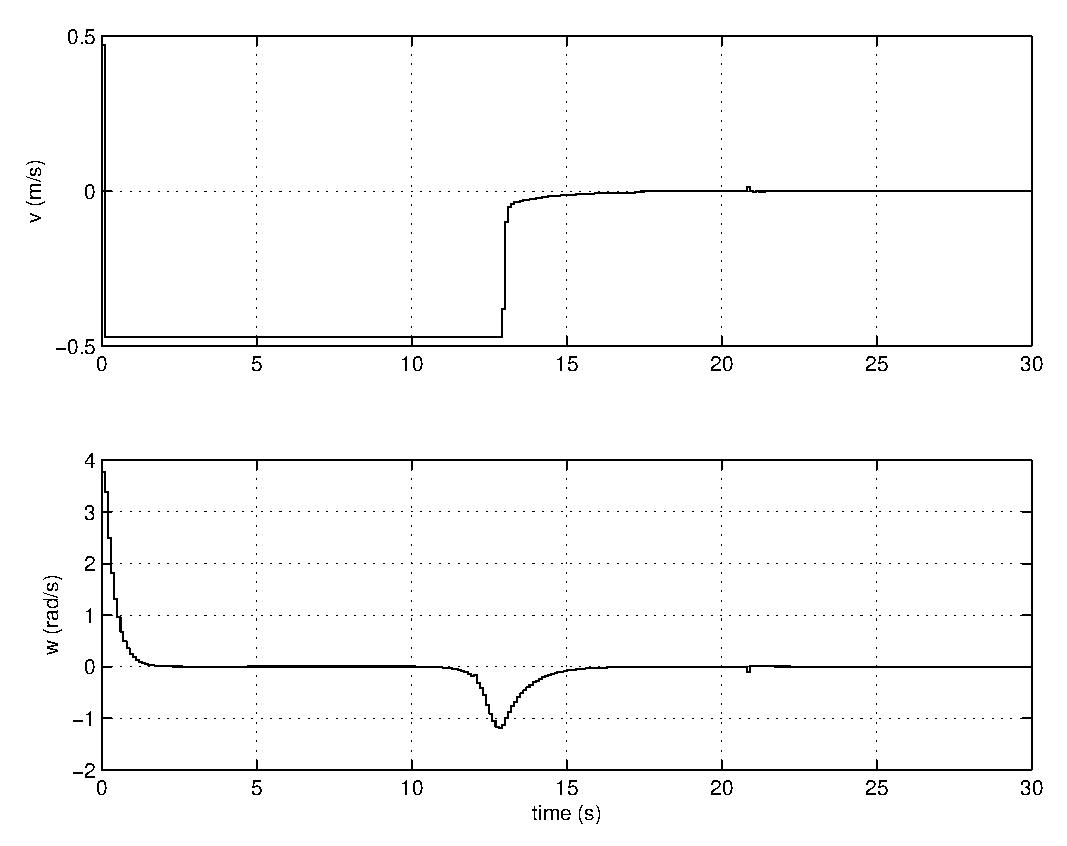
\includegraphics[width=.82\linewidth]{Figures/control_03.eps}
   	\caption{Control inputs.}
   	\label{fig:control_03}
\end{figure}

Comparing the results above with the results obtained in Section~\ref{sec:cartesian}, significative performance improvements with respect to both state and control trajectories can be noted. The robot needs about 16 s to achieve its objective, against 40 s and 21 s of the previous two cases, respectively. It can be seen in Fig.~\ref{fig:traj_03} that the $x$-state presents a maximum amplitude of about $0.3~m$, while for the example in Section~\ref{sec:essen} the $x$-state needs almost $3~m$ to maneuver towards the origin (Fig.~\ref{fig:traj_02}). Furthermore, in Fig.~\ref{fig:control_03} the control inputs are smoother than the ones presented in Fig.~\ref{fig:control_02}.

Also note that, with the transformation to polar coordinates, the decoupling between the position states $x$ and $y$ in the cost function has been possible. Now the final configuration is ${\bf x}_f=[0~~0~~0]^T$. Furthermore, it has been possible to improve the overall performance without the inclusion of another terms in the cost function or a longer prediction horizon. 

\subsection{NMPC with Constraints in Control and State Variables.}\label{sec:corridor}
In this section, we show an illustrative example of the WMR following a corridor. For such a task, the inclusion of constraints in the amplitude of the states such as~\req{eqn:restx} will be now considered in the optimization problem.

Then, by using the cost function in polar coordinates~\req{eqn:polar_cost} and the same control constraint and tuning parameters used in the previous examples and an initial condition of ${\bf x}_0=[-4~~4~~\pi]^T$, we obtain the result shown in Fig.~\ref{fig:traj_04}.
\begin{figure}[H]
	\centering
	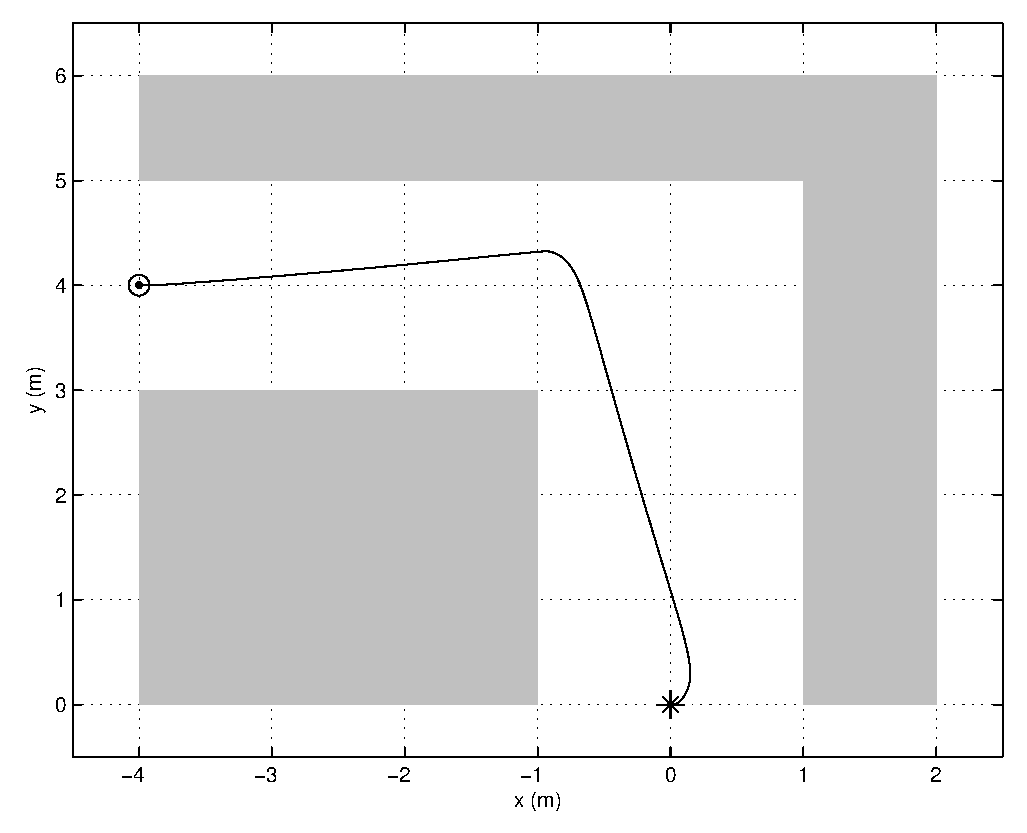
\includegraphics[width=.82\linewidth]{Figures/traj_04.eps}
   	\caption{Trajectory in the $XY$ plane.}
   	\label{fig:traj_04}
\end{figure}
%\begin{figure}[htbp]
%	\centering
%   	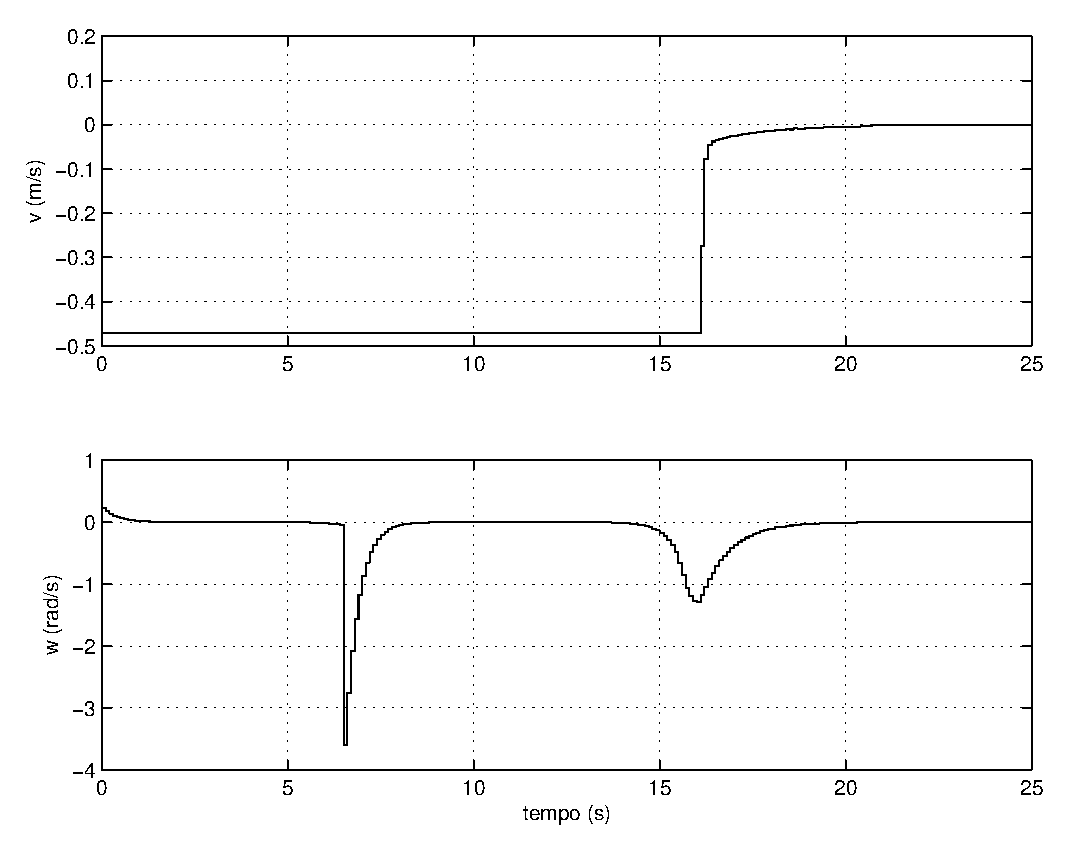
\includegraphics[width=.83\linewidth]{Figures/control_04.eps}
%   	\caption{Control inputs.}
%   	\label{fig:control_04}
%\end{figure}

Fig.~\ref{fig:traj_04} shows the trajectory of the robot in the XY-plane,
where the gray polygons stands for the walls of the corridor. It is
straightforward to note that the configuration space is non-convex which, for
an optimization problem such the one solved here, is
unacceptable~\cite{mayne00}. This problem can be overcome by splitting the
configuration space in two convex half-spaces and applying a {\em via-point
strategy}. Thus, different optimization problems are considered depending on
the value of $x(k|k)$. In the case presented here, $x=-1$ defines the limit
between the two half-spaces. For each half-space we consider the
problem~\req{eqn:optim}-\req{eqn:restu1} with different state constraints
and reference point ${\bf x}_r$ as follows:

\begin{equation*}
	\text{if}~x(k|k)<-1:
	\left\{
		\begin{aligned}
			&x(k+j|k)\leq 1, \\ 
			3\leq &y(k+j|k)\leq 5, \\
			&{\bf x}_r = [0~4~0]^T
		\end{aligned}
	\right.
\end{equation*}
\begin{equation*}
	\text{if}~x(k|k)\geq-1:
	\left\{
		\begin{aligned}
			-1\leq &x(k+j|k)\leq 1, \\ 
			&y(k+j|k)\leq 5, \\
			&{\bf x}_r = [0~0~0]^T
		\end{aligned}
	\right.
\end{equation*}
where ${\bf x}_r$ is the reference point which the robot must converge to.
%Further details of this approach can be seen in~\cite{kuhne05}.

\subsection{Comparison with Classical Approaches.}\label{sec:comp}
As pointed out in Section~\ref{sec:intro}, classical approaches to the control of nonholonomic WMRs include non-smooth and time-varying control laws. In this section a comparative analysis between the NMPC proposed here and some of these approaches are therefore carried out. The goal is once again the origin. For instance, let us consider the time-varying control of~\cite{samson91} and the non-smooth control of~\cite{canudas92}. Thus, with a initial condition of ${\bf x}_0=[-1~~3~~0]^T$ and considering control constraints~\req{eqn:const} in the NMPC, we have the results in Figures~\ref{fig:traj_05}-\ref{fig:control_05}, where the continuous line stands for the NMPC, the dashed line stands for the time-varying control law and the dash-dotted line stands for the non-smooth control law.

\begin{figure}[htbp]
	\centering
	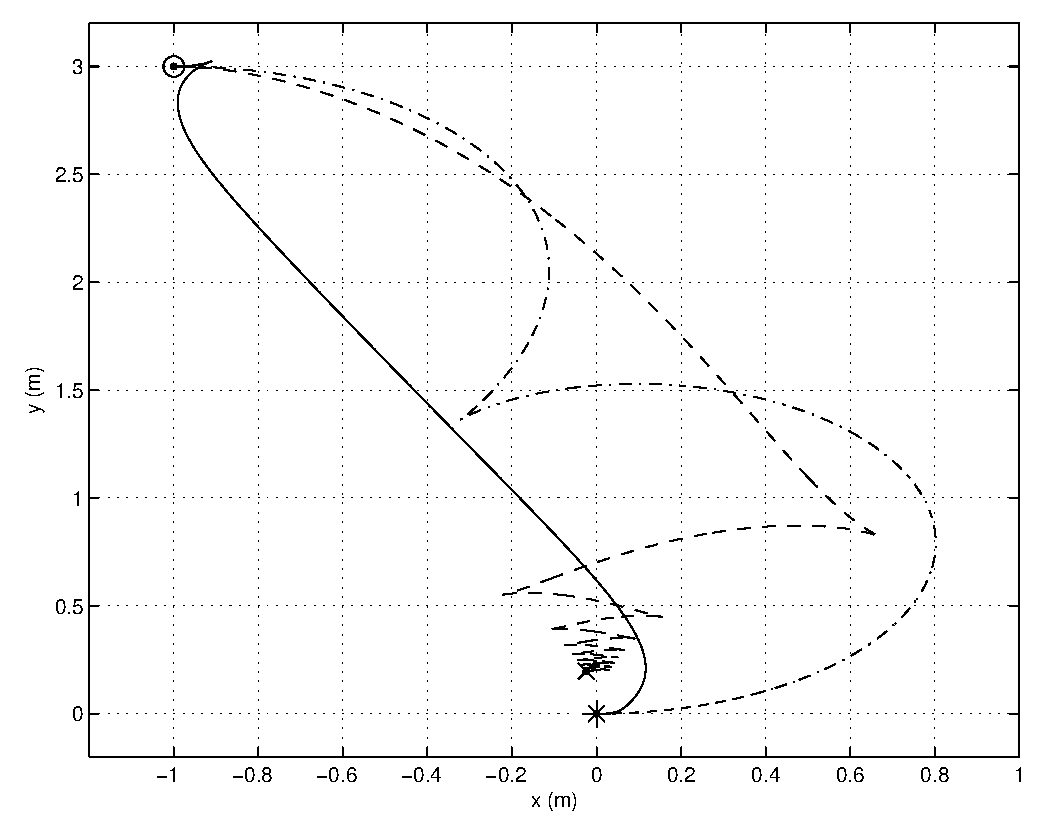
\includegraphics[width=.82\linewidth]{Figures/traj_05.eps}
   	\caption{Trajectory in the $XY$ plane.}
   	\label{fig:traj_05}
\end{figure}
\begin{figure}[htbp]
	\centering
   	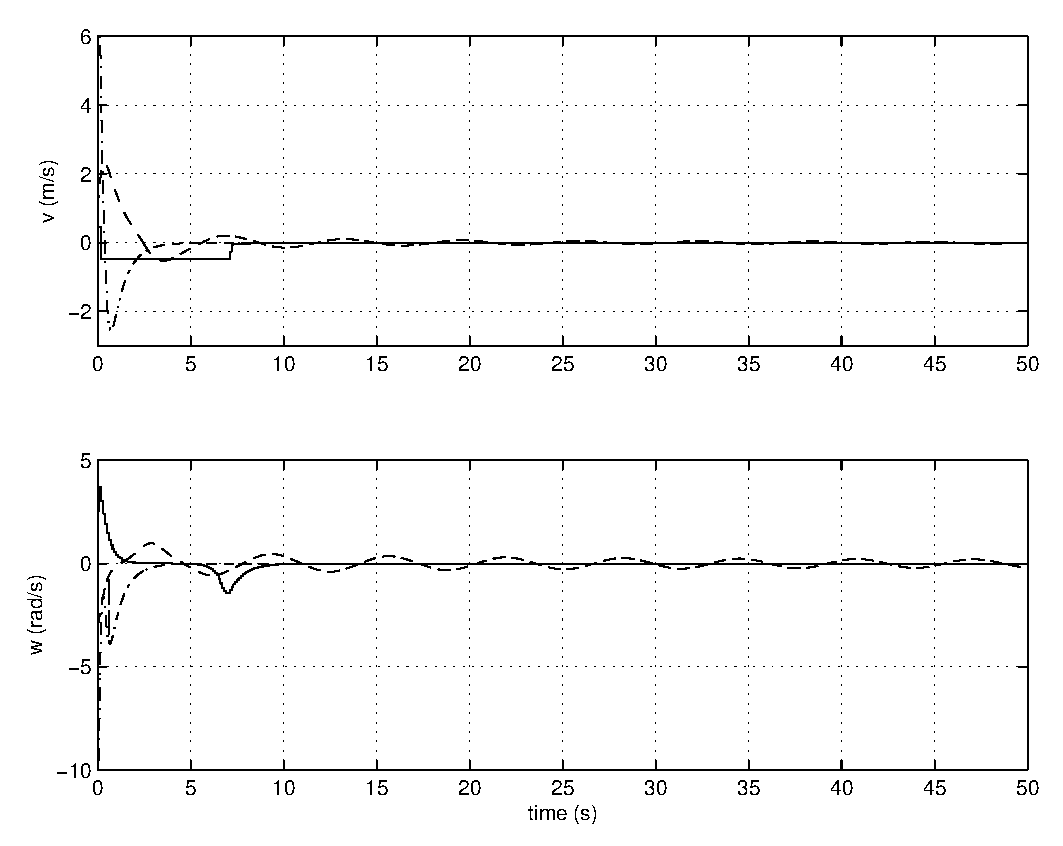
\includegraphics[width=.82\linewidth]{Figures/control_05.eps}
   	\caption{Control inputs.}
   	\label{fig:control_05}
\end{figure}

It is straightforward to note the typical features of the time-varying control law: low convergence rate and oscillatory movements. With the use of the non-smooth control, these problems can be avoided. 
However, the performance achieved with NMPC is even better. Furthermore, note in Fig.~\ref{fig:control_05} that the classical control laws violate the amplitude control constraints, while with the NMPC proposed here they are respected.

%%%%%%%%%%%%%%%%%%%%%%%%%%%%%%%%%%%%%%%%%%%%%%%%
\section{Computational Effort}\label{sec:effort}
The use of MPC for real-time control of systems with fast dynamics such as a WMR has been hindered for some time due to its numerical intensive nature. However, with the development of increasingly faster processors the use of MPC in demanding applications can be possible. 

In order to evaluate the real-time implementability of the proposed MPC, we consider, as measurement criterion, the number of floating point operations per second (flops). With this aim we consider that the computations run in an Athlon XP 2600+ which is able to perform a peak performance between 576 and 1100 Mflops accordingly to~\cite{aburto92}, a de-facto standard for floating point performance measurement. 

The data presented in Table~\ref{tab:comp} refers to the mean value of Mflops along the developed trajectory for the three examples above for a sampling period of $T=100~ms$. {\em Case 1} refers to the NMPC with the original cost function in cartesian coordinates~\req{eqn:cost}; {\em Case 2} is the NMPC with the cost function~\req{eqn:essen_cost} of~\cite{essen01}; and {\em Case 3} is the NMPC with the proposed cost function~\req{eqn:polar_cost}, in polar coordinates.

\begin{table}[htbp]
	\renewcommand{\arraystretch}{1.2}
	\centering
	\caption{Computational Effort.}
	\begin{tabular}{c|ccc}
	\hline
			& \multicolumn{3}{c}{Mflops} \\
	Horizon   & Case 1 & Case 2 & Case 3 \\
	\hline\hline
	5	& 6.41 & 14   & 8.17 \\
	10	& 114  & 384  & 128  \\
	12	& 246  & 926  & 434  \\
	15 	& 626  & 6077 & 1392 \\
	\hline
	\end{tabular}
	\label{tab:comp}
\end{table}

The data in Table~\ref{tab:comp} provides enough evidence that a standard of-the-shelf computer is able to run a MPC-based controller for a WMR. Note that for $N=5$ all of the examples are feasible in real-time. However, results presented in Section~\ref{sec:pure} show the existence of steady-state error and the results in Section~\ref{sec:essen} show poor performance. Thus, among all of them, the approach that performs the best results with respect to state and control trajectories and computational effort is the one proposed in Section~\ref{sec:polar}, the NMCP with cost function in polar coordinates.


%%%%%%%%%%%%%%%%%%%%%%%%%%%%%%%%%%%%%%%%%%%
\section{Conclusion}\label{sec:conclusions}

This paper has presented an application of model predictive control to the problem of point stabilization of a nonholonomic wheeled mobile robot. A steady-state error in one of the position variable has been identified and a transformation of the configuration variables into polar coordinates has been proposed and successfully solved the problem. Through some examples, it was shown an important advantage of MPC: it can handle constraints in a straightforward way. The obtained control signals were such that the constraints imposed on the control variables were respected. 

%As shown above, the choice of MPC for the application given here is well justified by some advantages: the existence of a performance criterion which is minimized, thus the control law is optimal with respect to this criterion; the straightforward way in which state/input constraints can be handled; the MPC implicitly generates a control law that deal with Brockett's conditions.

Furthermore, considerations regarding the computational effort of the MPC were developed with the purpose of speculating the viability of the proposed technique in a real implementation. It has been shown that with the proposed technique the NMPC can be potentially applied to WMRs in real-time.

\section*{Acknowledgments}
The authors gratefully acknowledge the financial support from CAPES and CNPq, Brazil.

% Equaliza as colunas da �ltima p�gina:
%\IEEEtriggeratref{5}

\bibliographystyle{IEEEtran}
\bibliography{icma05}

\end{document}
